\newpage
\chapter{Relazione tirocinio}
\label{cha:conclusioni}


In questo capitolo viene esposto un resoconto del tirocinio avvenuto tra i mesi di aprile e maggio 2019 presso il Liceo Galileo Galilei (Trento), il liceo Leonardo Da Vinci (Trento), l’istituto tecnico tecnologico Buonarroti-Pozzo (Trento) e il liceo Scientifico presso il collegio Arcivescovile Celestino Endrici (Trento). L’attività è stata strutturata in due parti: una parte teorica di lezione interattiva e una parte laboratoriale in cui i ragazzi svolgevano degli esercizi. Lo scopo del tirocinio è stato quello di proporre un modo diverso di visualizzare ed utilizzare l’informatica presso gli istituti superiori, seguendo i principi del modello Computational STEAM (\autoref{chap:steam}). L’argomento trattato, i protocolli epidemici (\autoref{chap:epidemic}), è stato scelto perché adatto a far comprendere come modelli e algoritmi studiati in altri campi (la biologia e la matematica) possano essere adattati ed utilizzati con efficacia in ambito informatico (nello specifico la comunicazione in sistemi distribuiti).
\section{Contesto}
Essendo tre studenti abbiamo organizzato questa esperienza di tironcio nel seguente modo: ognuno ha portato un argomento diverso, ma con le stesse modalità di presentazione (seguendo i principi di Computatonal STEAM) in tre classi per un totale di 9 classi.
Abbiamo presentato il corso tra aprile e maggio presso i seguenti istituti superiori: liceo Scientifico Galileo Galilei di Trento, liceo Scientifico Leonardo Da Vinci di Trento, liceo Scientifico collegio Arcivescovile Celestino Endrici e istituto tecnico e tecnologico Buonarroti-Pozzo. Abbiamo scelto questo periodo in quanto più adatto sia per i ragazzi che per gli insegnanti ordinari. Ci siamo concentrati sul liceo scientifico, in quanto il percorso di studi Computational STEAM è indirizzato a questa tipologia di scuola, ma abbiamo deciso di provare a portare l’esperienza anche in un istituto tecnico, per cercare di capire quali possono essere le differenze riguardo la preparazione dei ragazzi, in modo da adattare le lezioni al meglio. 

Il nostro obiettivo consisteva nel proporre dei corsi durante le ore di informatica, trattando tematiche che si interfacciassero ad altre materie studiate dai ragazzi. Dai dati raccolti abbiamo notato che questa metodologia, proposta sia all'interno della riforma Gelmini del 2010 \cite{riforma} sia tra i principi fondanti di Computational STEAM, spesso non è applicata: alcuni ragazzi conoscevano le potenzialità dell'informatica come scienza computazionale, mentre per altri è stata una novità. 

Le classi a cui sono rivolti sono terze, quarte e quinte, perché gli argomenti trattati risultano più adatti a studenti con conoscenze che vengono fornite a partire dal terzo anno in poi. La scelta delle classi è stata fatta dagli insegnanti di informatica, a cui sono stati proposti i moduli.


\section{Organizzazione del corso}
Abbiamo strutturato le lezioni nel seguente modo: un’ora per l’introduzione, e le restanti 6 ore per il contenuto del corso in sè. La lezione introduttiva e l’ultima sono state utilizzate anche per compilare un questionario introduttivo ed un conclusivo (entrambi anonimi), i cui risultati sono utilizzati come supporto alla stesura di questo capitolo. È stata utilizzata l’applicazione Moduli Google. Abbiamo raccolto le risposte di 164 ragazzi per il questionario iniziale, 161 per quello finale. Questi sono i dati aggregati per tutte le classi. Utilizziamo i dati aggregati per la parte  di contesto, mentre per la parte "tecnica" li suddividiamo in base al corso frequentato (alcune domande sono specifiche del modulo, come quelle riguardante il feedback riscontrato, il quale può variare in base a chi ha presentato il corso). 

Per quanto riguarda il corso sui protocolli epidemici, è stato distribuito in singole ore (da 50 minuti, come previsto per gli istituti superiori)ad eccezione dell'istituto tenico e tecnologico Buonarroti, in cui si è svolto in blocchi di 3 ore e un esperimento al liceo Da Vinci con una lezione di due ore, in cui è intervenuta la professoressa di scienze per portare alcune riflessioni riguardo la diffusione delle epidemie, spiegando quali sono state le pandemie piu' importanti della storia e come si sono diffuse. Abbiamo notato che svolgere le lezioni in blocchi di almeno due ore permette di approfondire maggiormente le tematiche affrontate, lasciando spazio ai ragazzi di completare gli esercizi. Con lezioni della durata di un'ora talvolta sgli studenti sono costretti a lasciare incompleti gli esercizi, per poi riprenderli l'ora successiva. 

\begin{figure}[!ht]
    \begin{subfigure}{.5\textwidth}
        \centering
        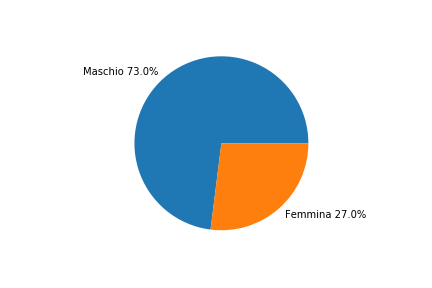
\includegraphics[width=\textwidth]{genere.png}
        \caption{Genere}
        \label{fig:genere}
    \end{subfigure}\hfill
    \begin{subfigure}{.5\textwidth}
        \centering
        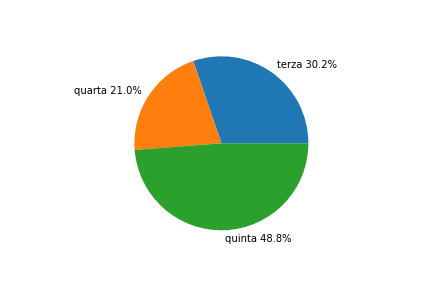
\includegraphics[width=\textwidth]{classi.png}
        \caption{Classi}
        \label{fig:classi}
    \end{subfigure}
    \caption{Caratteristiche del campione} 
\end{figure}
\subsection{Analisi del campione}
Le classi sono prevalente composte da maschi, il che non è affatto sorprendente osservando la composizione nei corsi di studio di informatica ed ingegneria. I ragazzi hanno notato questa differenza numerica, motivandola principalmente con questa affermazione: “l'informatica è preferita dai ragazzi”. Nonostante ciò, la figura dell’informatico è stata descritta in modo abbastanza lontano dai frequenti stereotipi: secondo i dati raccolti molti pensano che un informatico debba essere creativo e debba avere capacità nel lavorare in gruppo.

\begin{figure}[!ht]
    \centering
    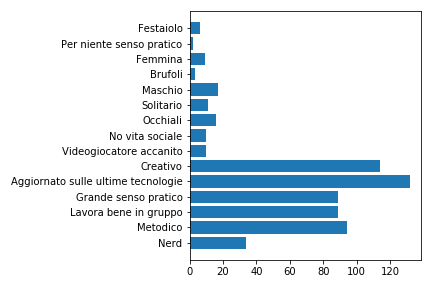
\includegraphics[height=8cm]{computer_scientist.png}
    \caption{Quali sono i requisiti per essere un perfetto informatico?}
    \label{fig:computer_scientist}
\end{figure}

Ai ragazzi è stato chiesto quanto apprezzano la materia in sè e come questa venga insegnata attualmente: i risultati presentano un giusto equilibrio, con alcuni studenti che la preferiscono ed altri che la disprezzano o non ne trovano l'utilità. Attraverso queste lezioni abbiamo cercato di trasmettere l'importanza dell'informatica, dimostrando che puo' rivelarsi divertente e interessante, senza ovviamente ricadere nella banalità.

\section{Contenuto e metodo esecutivo} 
Il contenuto del corso è stato esposto utilizzando delle slide per la parte di lezione teorica, mentre per la parte applicativa è stata fornita una cartella condivisa con gli esercizi da svolgere e le loro spiegazioni nel dettaglio (\href{http://www.tinyurl.com/protocolli-epidemici}{http://www.tinyurl.com/protocolli-epidemici}). Questo spazio è stato aggiornato durante il corso, aggiungendo nuovo materiale e correggendo errori e sviste notate dai ragazzi. All'interno si possono trovare, oltre alle istruzioni per una corretta installazione di Processing, un documento con la descrizione della libreria e degli esercizi da svolgere, il codice di partenza per eseguire gli esercizi, i lucidi proiettati durante le lezioni, il file compilato della libreria e una serie di link utili, per coloro che vogliono approfondire gli argomenti trattati (tra cui Processing e la diffusione delle epidemie) attraverso tutorial, articoli e libri. 

La parte teorica è stata presentata come lezione interattiva, dando spazio agli studenti di porci delle domande e di rispondere a quesiti da noi proposti. Ad eccezione della prima ora di lezione, tutte le altre hanno avuto una componente pratica, in modo tale che i ragazzi potessero applicare quanto imparato. La difficoltà degli esercizi è via via crescente, sia per la complessità degli algoritmi proposti, sia per un minore aiuto fornito in determinate situazioni (in alcuni casi è stato fornito solamente lo pseudocodice). 

\begin{figure}[!ht]
    \centering
    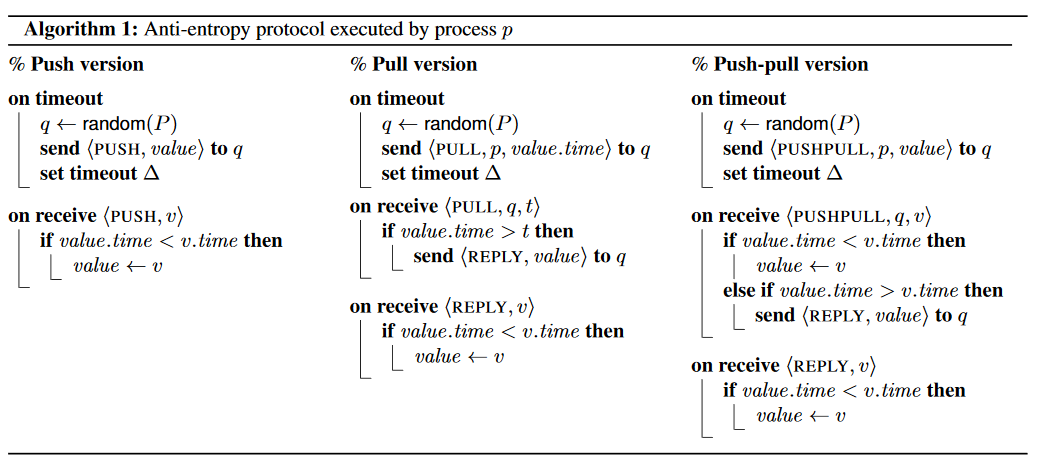
\includegraphics[width=.9\textwidth]{si_pseudocode.png}
    \caption{Esempi di pseudocodice presentati ai ragazzi \cite{montresor}}
    \label{}
\end{figure}

Tra i vari argomenti possibili ho scelto di sviluppare il corso sui protocolli epidemici (vedi \autoref{chap:epidemic}) per diversi motivi: in primo luogo, l’argomento si basa su semplici regole che vengono utilizzate più volte in diversi contesti. I protocolli di gossip possono però essere studiati maggiormente e lasciano spazio anche ad un approfondimento autonomo. Inoltre sono sono un argomento interdisciplinare: vengono utilizzati in reti distribuite per la comunicazione, ma i principi su cui si basano sono studiati in epidemiologia, nell’ambito quindi della diffusione delle epidemie, ma anche dalle scienze sociali, riguardo il fenomeno del gossip. Questa interdisciplinarietà si dimostra adatta all’interno di questa esperienza che vuole portare i principi di Computational STEAM nelle scuole superiori.

Nello specifico ho sviluppato il programma del corso nel seguente modo: nella prima lezione, utile come introduzione, ho presentato l’argomento e la sua natura interdisciplinare, il contesto storico, la definizione del problema, le applicazioni reali e i principi di base.
\begin{figure}[!ht]
    
    \begin{subfigure}{.5\textwidth}
        \centering
        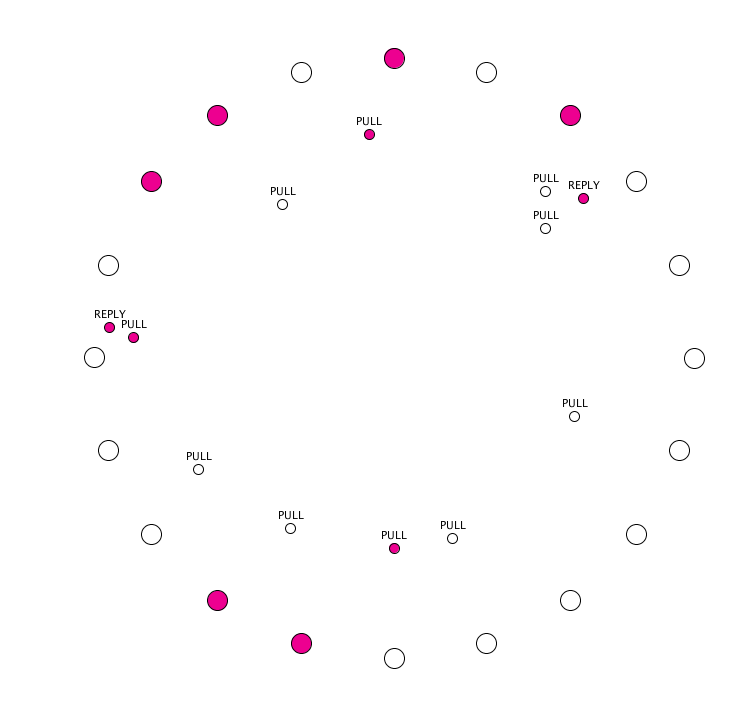
\includegraphics[width=\textwidth]{pull.png}
        \captionsetup{justification=centering}
        \caption{Algoritmo modello SI: pull} 
    \end{subfigure}\hfill
    \begin{subfigure}{.5\textwidth}
        \centering
        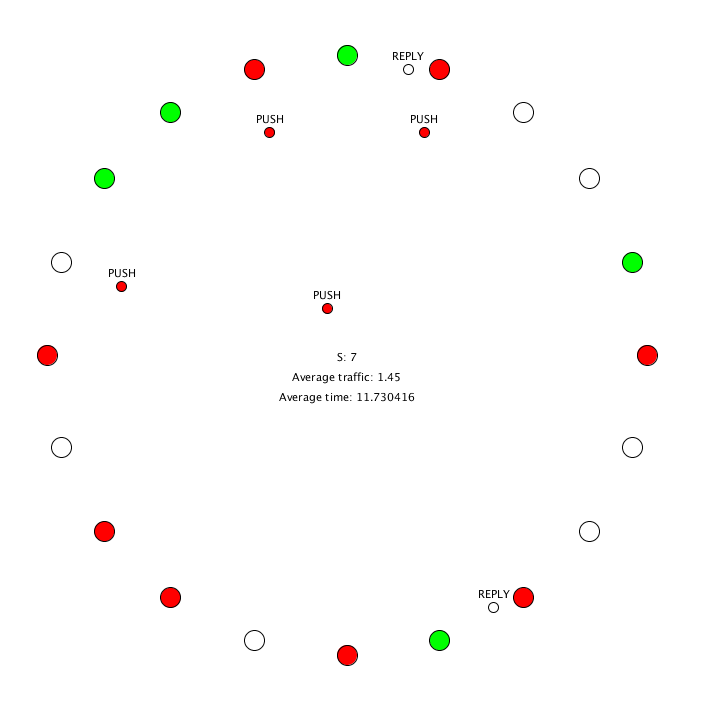
\includegraphics[width=\textwidth]{feedback-counter.png}
        \captionsetup{justification=centering}
        \caption{Algoritmo modello SIR: Feedback-Counter} 
    \end{subfigure}
    \caption{Esempi di output}
    \label{fig:output}
\end{figure} 

Nelle successive lezioni mi sono concentrato, dopo aver fatto una breve introduzione sui grafi (utile per alcune definizioni), sui due modelli SI e SIR presentando gli algoritmi e stili che li utilizzano, lasciando poi spazio ai ragazzi di implementarli su schermo. Nello specifico i ragazzi hanno completato esercizi riguardo gli stili Push, Pull e Push-Pull per il modello SI, e le varianti Feedback-Counter e Blind-Coin per quanto riguarda il modello SIR. ho preparato un esercizio su Aggregazione, che per mancanza di tempo non e' stato possiblie esporre.

Una lezione tipo è stata organizzata nel seguente modo: nella prima parte viene introdotto il modello e viene definito il problema. Poi vengono introdotte le componenti necessarie, i metodi della libreria utili per la risoluzione. Infine viene esposto lo pseudocodice, che suddivide i momenti fondamentali dell'esecuzione degli algoritmi: allo scadere del timer e alla ricezione delle informazioni. Nel tempo restante della lezione i ragazzi cercano di trovare una soluzione al problema, completando gli esercizi (l'output di alcuni esercizi in Figura \ref{fig:output}).

L’ambiente di sviluppo utilizzato è Processing (\href{https://processing.org}{https://processing.org}), libreria grafica di Java e IDE utile per creare simulazioni e metodi di visualizzazione efficace \cite{processing_wikipedia}. La versione utilizzata è la 3.5.3: è stata installata prima dell'inizio del corso sulle macchine dei laboratori con sistema operativo Windows 10.

Ho fornito una libreria (\href{https://github.com/ainter21/epidemic}{https://github.com/ainter21/epidemic}), utile sia per alleggerire il carico di lavoro, sia per nascondere alcune componenti troppo complesse, come la parte di visualizzazione (lo scopo degli esercizi è quello di implementare l’algoritmo, mentre la parte di visualizzazione è solamente un supporto per rendere più chiari i concetti).
Ho fornito la documentazione utile per completare gli esercizi, con la spiegazione dei metodi e degli attributi. Il loro obiettivo è stato quindi utilizzare la libreria fornita (con metodi molto simili a quelli utilizzati nell' pseudocodice), affinché gli algoritmi proposti funzionassero. La lista degli esercizi proposti già completati è scaricabile qui (\href{https://github.com/ainter21/epidemic-protocols}{https://github.com/ainter21/epidemic-protocols}).

Le attività sono state svolte nei laboratori di informatica, in modo tale da poter proiettare i lucidi e permettere ai ragazzi di lavorare in autonomia o a gruppi. L'idea iniziale era di formare dei gruppi di lavoro per poter collaborare e sviluppare abilità di problem solving e lavoro di squadra. Questa soluzione si è rivelata di difficile attuazione in quanto i ragazzi possiedono un account personale non condivisibile e se alcuni studenti rimanevano assenti, si rischiava di non poter accedere al lavoro iniziato la volta precedente. Abbiamo comunque fatto il possibile per invogliarli a lavorare in gruppo.

\subsection{Libreria nel dettaglio}
La libreria è stata scritta in modo tale da nascondere la parte di programmazione ad oggetti non studiata dai ragazzi al liceo scientifico. Le classi principali sono: \texttt{Graph}, \texttt{Node} e \texttt{Info}. La rete è visualizzata attraverso un grafo. Ho associato il valore interno del nodo ad un colore, per rendere l'output visivo piú accattivante.

I ragazzi hanno utilizzato i metodi già implementati nei vari oggetti (specialmente nella classe \texttt{Node}) per eseguire azioni e acquisire informazioni. Il grafo creato è completo, assunzione che durante le lezioni non è stata rilassata per mancanza di tempo.

All'interno della libreria è presente una classe astratta \texttt{Graph}, da cui sono definiti grafi dei rispettivi modelli: \texttt{GraphSI}, \texttt{GraphSIR} e \texttt{GraphAggregation}. Vengono inizializzati come grafi completi, in quanto durante il corso è stata fatta questa assunzione. Ogni grafo ha un metodo utilizzato per aggiornare le sue componenti \texttt{updateGraph()} ed uno per disegnarlo ad ogni frame di esecuzione \texttt{drawGraph()}. 

La seconda classe, \texttt{Node}, oltre al metod per disegnarla \texttt{drawNode()}, è fornita di metodi utili per aggiornare il valore (\texttt{setValue()}, \texttt{setInfected()} e \texttt{setRemoved()}), per resettare il timer interno \texttt{reseTimer()} e per inviare le informazioni \texttt{sendInfo(target, type)}. Quest'ultimo metodo istanzia un ulteriore oggetto, \texttt{Info}, utile per contenere tutti i dati che devono essere poi processati nel momento in cui l'informazione arriva a destinazione (secondo gli algoritmi e i modelli spiegati nel \autoref{chap:epidemic}).

I ragazzi hanno comunque avuto la possibilità di leggere il codice e di modificarlo, compilando la propria versione della libreria.
\section{Analisi dei risultati}

\begin{figure}[ht]
    
    \begin{subfigure}{.5\textwidth}
        \centering
        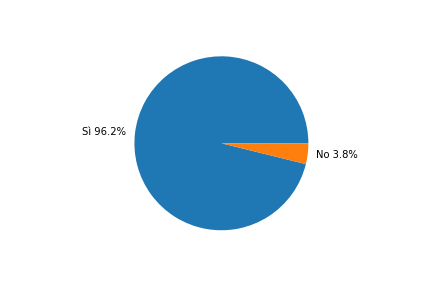
\includegraphics[width=\textwidth]{aspettative.png}
        \captionsetup{justification=centering}
        \caption{Ritieni che siano state \\ soddisfatte le tue aspettative?} 
    \end{subfigure}\hfill
    \begin{subfigure}{.5\textwidth}
        \centering
        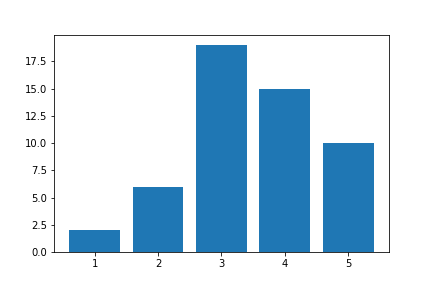
\includegraphics[width=\textwidth]{conoscenze.png}
        \captionsetup{justification=centering}
        \caption{Quanto il corso era adatto  \\ al tuo livello di conoscenze?} 
    \end{subfigure}
    \caption{Risultati}
\end{figure} 

Dopo le sette ore previste, abbiamo chiesto di compilare un questionario di valutazione delle attività svolte.  I dati analizzati in questa sezione non sono i dati aggregati: 60 risposte per il questionario iniziale, e 52 per il questionario finale, ovvero quelle riguardanti il modulo "protocolli epidemici".

I risultati sono positivi, la maggior parte degli studenti dice di essere rimasto soddisfatto. Gli argomenti trattati erano una novità per la maggior parte dei ragazzi, ed alcuni hanno riferito di voler approfondire l'argomento (sia per quanto riguarda l'utilizzo di Processing, sia per i protocolli epidemici, sia per la diffusione delle epidemie). 

Avendo portato il corso sia in un liceo che in un istituto tecnico abbiamo notato alcune differenze, a causa del programma svolto dai ragazzi e dal numero di ore assegnate all'informatica. I ragazzi del liceo, non avendo programmato ad oggetti, si sono trovati in difficoltà nel comprendere alcuni concetti. Conoscevamo già il programma svolto ed il livello di preparazione, ma abbiamo comunque optato per l'utilizzo di Processing e quindi di Java, in quanto avrebbe reso piú accattivante il risultato finale per i ragazzi. Alcuni ragazzi hanno avuto piú difficoltà nel lavorare in gruppo perché, da quanto capito, non è una tecnica molto utilizzata durante l'anno. Inoltre si sono trovati spaesati nel momento in cui abbiamo dato loro autonomia nello svolgere gli esercizi: alcuni hanno avuto difficoltà nel completare gli esercizi. Ai ragazzi è stato suggerito di scrivere su carta, riflettere in gruppo per cercare una possibile soluzione, ma questo consiglio non è stato molto seguito e la maggior parte ha iniziato a scrivere immediatamente codice, con risultati non sempre soddisfacienti. In alcuni casi è stato mostrato dello pseudocodice in modo da dare un punto di partenza: all'istituto tecnico era già stato utilizzato questo metodo, quindi questo materiale è risultato piú utile.

Anche l'utilizzo di una libreria è stata una novità per i ragazzi: hanno sperimentato questa potenzialità dei linguaggi di programmazione consultando la documentazione fornita, cercando di capire quali metodi e attributi fossero adatti alla situazione. Anche se all'inizio si sono trovati un po' spaesati, con il procedere del corso hanno preso dimestichezza con il metodo proposto.

Sarebbe stato anche utile investire alcune ore per introdurre in modo piú approfondito l'ambiente di sviluppo, ma purtroppo il tempo era limitato e questo avrebbe ridotto lo spazio dedicato all'argomento principale del corso. Il codice Processing può essere scritto in diversi linguaggi di programmazione oltre a Java: Python e Javascript. Si potrebbe provare a portare questi corsi utilizzando il linguaggio Python, piú semplice rispetto a Java (è stato scelto Java perché simile al C++, utilizzato durante l'anno dai ragazzi). Python presenta alcuni vantaggi rispetto ad altri linguaggi, specialmente nel contesto degli istituti superiori: come viene fatto notare da Grandell e colleghi in \cite{python_high_school}, questo linguaggio ha una sintassi piú semplice rispetto ai linguaggi normalmente utilizzati, è tipizzato dinamicamente (può essere uno svantaggio, ma riduce la quantità di codice) ed oggigiorno è sempre piú utilizzato anche nel mondo del lavoro. Inoltre le potenzialità di Python emergono anche dal grande numero di moduli che possono essere aggiunti. 

In conclusione si può dire che l'esperienza ha avuto esito positivo leggendo i feedback dei ragazzi ed è stato utile a noi per capire in che modo proporre un argomento esterno al programma scolastico presentandolo con modalità diverse da quelle classiche. è stato utile ai ragazzi per capire come l'informatica possa essere applicata ed utilizzata come materia interdisciplinare e di supporto e come altre materie si possono interfacciare all'informatica (Vedi Tabella \ref{table:risposte_finali}). Nel caso venga riproposta un'esperienza simile, è auspicabile che i ragazzi abbiano già un conoscenza di base riguardo la programmazione ad oggetti e l'ambiente di sviluppo Processing in modo da rendere piú comprensibili alcuni concetti e dare piú libertà ai ragazzi nello scrivere il codice (il dover partire da zero a scrivere il codice leggendo la documentazione della libreria è stato uno scoglio troppo grande da superare, quindi gli esercizi sono stati presentati in modo guidato, cone delle parti da completare).



\begin{center}
\def\arraystretch{1.5}
\begin{table}[!ht]

    \caption{Alcune risposte date dai ragazzi nel questionario finale}

    \begin{tabular}{p{.9\textwidth}}
        
        \bfseries{Hai cambiato idea su qualcosa riguardo all'informatica dopo questi incontri?} \\
        \midrule
        "Ho scoperto che può essere anche molto divertente"  \\
        "ho conosciuto delle sue applicazioni molto interessanti" \\
        "Si, che l'informatica può essere applicata in diversi ambiti" \\
        "Ho cambiato idea sull'applicazione dell'informatica in campi diversi, penso che sia un buon supporto!" \\
        "Si è riaffermato in me il concetto che l'informatica non abbia confini, in termini di campi di applicazione." \\
        \midrule
        \bfseries{Ci sono state cose che non hai capito o che sono state spiegate in modo poco chiaro?} \\
        \midrule
        "La sintassi non è stata introdotta e sarebbe stato ideale" \\
        "alcune parti di programmazione" \\
        "Non in particolare, forse avrei avuto bisogmo di qualche spiegazione in più rispetto al codice" \\
        "In generale il funzionamento di java a mio parere non è stato trattato abbastanza" \\
    \end{tabular}
    \label{table:risposte_finali}
\end{table}


\end{center}